%% Source: https://github.com/tias/constraint-solving-course
%% Licensed under CC BY-NC-SA 4.0: https://creativecommons.org/licenses/by-nc-sa/4.0/
%% You may share and adapt this for non-commercial use,
%% with attribution and under the same license.

\documentclass{cons-beamer}
\usepackage{cancel}

\begin{document}

% Teach BEWARE: this lecture probably takes 3 hours (split into next?)
\titleFrame{
	L03: Global Constraints
}{
	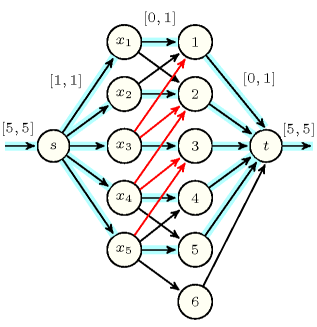
\includegraphics[height=42mm]{images/flow_alldiff_only_graph.png}
}{
	Partly based on slides from Pierre Flener and Dimos Tsouros.
}


\section{Motivation and definition}

\begin{frame}{First: primitive constraints and propagation}
	From Lecture 1:\\
	Solving combinatorial problems \textbf{intelligently}:
	\begin{itemize}
		\item \search{Search}: Explore the space of possible assignments.
		\item \inference{Inference}: Reduce the space to feasible (partial) assignments.
	\end{itemize}
	\vfill

	In this lecture we refine \textit{how} solvers do inference:
	\pause
		
	\begin{definition}
		\textit{Primitive constraint}: a constraint that the solver can do  \inference{inference} with.
	\end{definition}
	
	For CP, PB and SAT inference=\inference{propagation}.
	
	\begin{definition}
		\textit{Propagation}: using the properties of a primitive constraint to \inference{reduce the domains} of participating decision variables by removing unsupported values.
	\end{definition}
	Example: $x + 2 \cdot y \geq 3, \quad D(x) = \{0,1,2\}, D(y) = \{0,1,2\}$ \\
	$\qquad \qquad \qquad \implies D(y) = \{\cancel{\red{0}},1,2\}$
\end{frame}

\begin{frame}{Solvers and primitive constraints}
	Different solver paradigms have different \defined{primitive} constraints:
	\vfill
	
	\begin{itemize}\setlength\itemsep{1em}
		\item \textbf{Boolean SATisfiability solvers}: Clause: $b_1 \vee b_2 \vee ... \vee b_n$
		\item \textbf{Pseudo-Boolean solvers}: $\sum w \cdot b \;\lessgtr\; c$ \\
			\quad(with $w,c$ constant, $\;\lessgtr\; \in \{=,<,\leq,>,\geq\}$)
		\item \textbf{Integer Linear solvers}: $\sum w \cdot v \;\lessgtr\; c$ and $v \;\lessgtr\; c$ \\
			\quad(with $w,c$ constant, $\;\lessgtr\; \in \{=,\leq,\geq\}$)
	\end{itemize}
	\vfill
	
	\textbf{CP solvers} have all-of-the-above + $\neq$ + \textit{global constraints}
\end{frame}

% This is more a thought exercise for me
\iffalse
\begin{frame}{Minimal set of primitive constraints for CP solver}
	\textbf{Required}
	\begin{itemize}
		\item Clause: $b_1 \vee b_2 \vee ... \vee b_n$
		
		\item Basic comparison: $v \;\lessgtr\; c$ with $\;\lessgtr\; \in \{=,\neq,<,\leq,>,\geq\}$ \\ 
		\qquad (canonical $\;\lessgtr\; \in \{=,\neq,\leq,\geq\}$)
		
		\item Implied basic comparison: $b \rightarrow (v \;\lessgtr\; c)$ with $\;\lessgtr\; \in \{=,\neq,<,\leq,>,\geq\}$ \\ \qquad (canonical $\;\lessgtr\; \in \{=,\neq,\leq,\geq\}$)
		
		\item Linear: $\sum w*v \;\lessgtr\; c$ with $\;\lessgtr\; \in \{=,\neq,<,\leq,>,\geq\}$ \\ \qquad (canonical $\;\lessgtr\; \in \{=,\neq,\leq\}$)
	\end{itemize}
	
	\textbf{Recommended}
	\begin{itemize}
		\item Element: $\cons{ElementEq}{Arr,idx,res}$
		
		\item AllDifferent: $\cons{AllDifferent}{V}$
		
		\item Implied linear: $b \rightarrow (\sum w*v \;\lessgtr\; c) $ with $\;\lessgtr\; \in \{=,\neq,<,\leq,>,\geq\}$ \\
		\qquad (canonical $\;\lessgtr\; \in \{=,\neq,\leq\}$)
		
		%\item Boolean linear: $\sum w*b \;\lessgtr\; c$ with $\;\lessgtr\; \in \{=,\neq,<,\leq,>,\geq\}$ \\ \qquad (canonical: $\;\lessgtr\; \in \{=,\neq,\leq\}$)
		
		\item Cumulative: $\cons{Cumulative}{S, D, R, c}$ \qquad (for scheduling)
		
		\item Other: \cons{Table}{}, \cons{MinimumEq}{}, \cons{MultiplyEq}{}, \cons{AbsEq}{}
	\end{itemize}
\end{frame}
\fi

\begin{frame}
  \begin{definition}
    \textit{Global Constraint}: a named constraint that represents a non-trivial relationship between decision variables.
  \end{definition}
  \vfill
  
  They are typically used to represent a specific combinatorial substructure commonly found in constraint satisfaction problems.
  \vfill
  
  \begin{example}
    Well-known global constraints
    \begin{itemize}
      \item \cons{AllDifferent}{}
      \item \cons{Circuit}{}
      \item \cons{NoOverlap}{}
      \item \dots
    \end{itemize}
  \end{example}
\end{frame}

\begin{frame}{Modeling with global constraints}
	
	When you write a model with global constraints:
	
	\begin{enumerate}
		\item If the solver has this global constraint as a \defined{primitive constraint}: it will use its propagator to eliminate values during search
		
		\item If the solver does not have it as primitive constraint: the constraint needs to be \defined{decomposed} and rewritten into primitive constraints. This often involves additional 'auxiliary' decision variables.
	\end{enumerate}
	\vfill
	
	\begin{definition}
		\textit{Decomposition:} rewriting a constraint into an equivalent set of simpler constraints
	\end{definition}
	\vfill
	
	A constraint modeling system will, for a chosen target solver, decompose and rewrite constraints until only primitive constraints remain.
\end{frame}


\begin{frame}{Why use Global Constraints?}
  \begin{itemize}
    \item[+] \textbf{Expressiveness}! \\
      More compact and intuitive models, closer to problem definition. \\ 
      Many expressive global constraints available \vfill 
      \begin{itemize}
        \item \textbf{Simplified modeling}: Global constraints enable the modeler to express complex conditions simpler. \\
              Simpler modeling reduces the chance of modeling errors.

        \item \textbf{Compactness}: Instead of writing multiple smaller constraints, a single global constraint can capture the entire logic. \\
              Makes the model more intuitive and readable
      \end{itemize}
  \end{itemize}
  \vfill

  \begin{example}
    Task allocation: I want all tasks to be allocated to a different team. \\
    \begin{itemize}
      \item \textit{Without global}: \\
            $Task_0 \neq Task_1, \; Task_0 \neq Task_2, \; Task_1 \neq Task_2, \; \dots$
      \item \textit{With global}: \cons{AllDifferent}{Task}
    \end{itemize}
  \end{example}
\end{frame}

\begin{flashcardcpmpy}
\begin{frame}{Why use Global Constraints? -- CPMpy}
  \begin{itemize}
	\item[+] \textbf{Expressiveness}! \\
	More compact and intuitive models, closer to problem definition. \\ 
	Many expressive global constraints available \vfill 
	\begin{itemize}
		\item \textbf{Simplified modeling}: Global constraints enable the modeler to express complex conditions simpler. \\
		Simpler modeling reduces the chance of modeling errors.
		
		\item \textbf{Compactness}: Instead of writing multiple smaller constraints, a single global constraint can capture the entire logic. \\
		Makes the model more intuitive and readable
	\end{itemize}
  \end{itemize}
  \vfill

  \begin{example}
    Task allocation: I want all tasks to be allocated to a different team\\
    \begin{itemize}
      \item \textit{Without global}: \\ \cpminline{Task[0] != Task[1], Task[0] != Task[2], Task[1] != Task[2],} \dots \\
      \item \textit{With global}:  \cpminline{cp.AllDifferent(Task)}
    \end{itemize}
  \end{example}
\end{frame}
\end{flashcardcpmpy}

\begin{frame}{Why use Global Constraints?}
  \begin{itemize}
    \item[+] \textbf{Efficiency}! (If available as primitive constraint) \\
             Faster solving, due to better \inference{inference} (stronger
             \inference{propagation}), enabled by more global information in
             the model
             \begin{itemize}
               \item More global information in one constraint can result to advanced filtering of the \search{search} space
               \item Specialized algorithms to detect \conflict{conflicts} faster during search.
             \end{itemize}
  \end{itemize}
  \vfill

  \begin{example}
    \textbf{Task allocation}: I want to allocate $n$ tasks to $m$ teams, s.t. each task is assigned to a different team. Assume we have $m < n$. \\
    \begin{itemize}
      \item \textit{Without global}: Each $\neq$ constraint needs 2 values (teams) available for its tasks. Will realize that there are not enough values only after extensive search of possible assignments \\
      \item \textit{With global}: \cons{AllDifferent}{Task} will directly recognise that we cannot put $m$ different values (teams) in $n$ variables (tasks) if we have $m < n$ during search. $\leftarrow$ \textit{Pigeonhole principle}
    \end{itemize}
  \end{example}
\end{frame}

\begin{frame}{Modelling with Global Constraints:}
  \vfill
  
  Many global constraints exist, capturing different combinatorial properties: \\
  Global-Constraint Catalogue \url{https://sofdem.github.io/gccat}
  \vfill

  \textbf{Functional Global Constraints}: Global constraints that have a functional component, such as \cons{MinimumEq}{}, \cons{MaximumEq}{}, \cons{CountEq}{}, \cons{NValueEq}{}, etc.
  \vfill

  \begin{definition}
    A global constraint \cons{G}{V} is \textit{functional} if and only if there exists a partitioning of the arguments $V$ into two non-empty and non-overlapping subsets $V1, V2$, such that \textit{the assignment of decision variables in subset $V2$ is defined using a function on the subset $V1$}.
  \end{definition}
\end{frame}

\begin{frame}{Modelling with Global Constraints:}
  \vfill

  \begin{definition}
    A global constraint \cons{G}{V} is \textit{functional} if and only if there exists a partitioning of the arguments $V$ into two non-empty and non-overlapping subsets $V1, V2$, such that \textit{the assignment of variables in subset $V2$ is defined using a function on the subset $V1$}.
  \end{definition}
  \vfill

  In many cases, this involves associating the value of the functional component with a variable:

  \begin{examples}
    \begin{itemize}
      \item \cons{MaximumEq}{X, v} expresses that $v = \cons{Maximum}{X}$. Now, $v$ can be used in other expressions.
      \item \cons{MinimumEq}{X, v} expresses that $v = \cons{Minimum}{X}$.
      \item \dots
    \end{itemize}
  \end{examples} 
\end{frame}

\begin{flashcardcpmpy}
\begin{frame}{Modelling with Global Constraints -- CPMpy}
  \begin{itemize}
    \item A number of commonly-used \defined{global constraints} are available in CPMpy: \\ \cpminline{AllDifferent, AllEqual, Cumulative, Table,} \dots
      \begin{footnotesize}
        API documentation: \\ \url{http://cpmpy.readthedocs.io/en/latest/api/expressions/globalconstraints.html}
      \end{footnotesize}
     \vfill
      
     \item All global constraints can be reified - be nested in other expressions: e.g. \\
        \cpminline{cp.sum(cp.AllDifferent(x), cp.AllDifferent(y), cp.AllDifferent(z)) > 2}
    \vfill
    
    \item A number of commonly-used \defined{global functions} are available too, representing only the \textit{functional} component: e.g. \cpminline{cp.Maximum(X)}
    \begin{itemize}
      \item Can be used nested in any expression: e.g. \cpminline{cp.Maximum(X) < 10}
      \item Several Global functions available: \\ \cpminline{Maximum, Minimum, Count, NValue,} \dots 
        \begin{footnotesize}
          API documentation: \\ \url{http://cpmpy.readthedocs.io/en/latest/api/expressions/globalfunctions.html}
        \end{footnotesize}
    \end{itemize}
  \end{itemize}
\end{frame}
\end{flashcardcpmpy}


\section{Counting over integer values}

\subsection{\cons{AllDifferent}{} and \cons{NValueEq}{}}

% From Peter: AllDifferent is the combinatorial structure of a basic assignment problem
\begin{frame}{\cons{AllDifferent}{}}
  \begin{definition}[Lauri\`ere, 1978]
    The \cons{AllDifferent}{X} constraint holds if and only if all the elements of array $X$ take distinct values.
  \end{definition}
  
  Its \defined{decomposition} is a conjunction of $\frac{n \cdot (n-1)}{2}$ disequality constraints \\
  when \( X \) has \( n \) elements:
  \begin{align*}
  	&X_i \neq X_j  &\forall i, j \in \{1, \ldots, n\}, i < j
  \end{align*}
  \vfill

  \begin{examples}
    \begin{itemize}
      \item Sudoku, Room assignment, Task allocation, \dots
    \end{itemize}
  \end{examples}
  \vfill
  \pause

  Variant: The \cons{AllDifferentExceptN}{X, N} constraint allows multiple occurrences of the excepted value $N$ only (e.g. except $0$).
\end{frame}
% FROM LATER SLIDES, CONJUNCTION NOTATION
%\begin{example}
%	\small
%	$\cons{AllDifferent}{x_1, \dots, x_n}$:
%	Its decomposition is a conjunction of
%	$\frac{n\cdot(n-1)}{2}$ disequality
%	constraints:
%	\vspace{-3mm}
%	\[
%	\bigwedge_{i, j \in \{1..n\}, i < j} x_i \neq x_j
%	\]
%\end{example}

\begin{flashcardcpmpy}
\begin{frame}{\cons{AllDifferent}{} -- CPMpy}
  \begin{definition}[Lauri\`ere, 1978]
  	The \cons{AllDifferent}{X} constraint holds if and only if all the elements of array $X$ take distinct values.
  \end{definition}
  Its decomposition is a conjunction of \(\frac{n \cdot (n-1)}{2}\) disequality constraints \\
  when \( X \) has \( n \) elements:
  \begin{center}
	\begin{tabular}{@{}ll@{}}
		\textbf{Math:} &
		\begin{minipage}[t]{0.75\linewidth}
			\vspace{-1.25em}
			\[
				X_i \neq X_j  \qquad \qquad \forall i, j \in \{1, \ldots, n\},\ i < j
			\]
		\end{minipage}
		\\
		\textbf{CPMpy:} &
		\begin{minipage}[t]{0.75\linewidth}
			\vspace{-0.7em}
			\cpminline{model.add( var1 != var2 for var1, var2 in all_pairs(X) )}
		\end{minipage}
	\end{tabular}
  \end{center}
  \vfill

  Variant: The  \cpminline{cp.AllDifferentExceptN(X, N)} constraint allows multiple occurrences of the excepted value $N$ only (e.g. except $0$).
\end{frame}
\end{flashcardcpmpy}

\begin{frame}
  \begin{example}
    Sudoku: we want distinct values in rows, columns and blocks.\\
    Using the \cons{AllDifferent}{X} global constraint:
    \begin{align*}
      &\text{AllDifferent}(\{G_{ij} \mid j \in \{1, \ldots, 9\}\}) & & \forall i \in \{1, \ldots, 9\} \quad \text{(rows)} \\
      &\text{AllDifferent}(\{G_{ij} \mid i \in \{1, \ldots, 9\}\}) & & \forall j \in \{1, \ldots, 9\} \quad \text{(columns)} \\
      &\text{AllDifferent}(\{G_{kl} \mid k \in \{i, \ldots, i+2\}, l \in \{j, \ldots, j+2\}\}) & & \forall i, j \in \{1, 4, 7\} \quad \text{(blocks)}
    \end{align*}

    The above is more expressive (and efficient) than using binary not equal constraints:
    \begin{align*}
      &G_{ij} \neq G_{ik} & \quad & \forall i \in \{1, \ldots, 9\}, \, \forall j, k \in \{1, \ldots, 9\}, \, j < k \quad \text{(rows)} \\
      &G_{ij} \neq G_{kj} & \quad & \forall j \in \{1, \ldots, 9\}, \, \forall i, k \in \{1, \ldots, 9\}, \, i < k \quad \text{(columns)} \\
      &G_{kl} \neq G_{mn} & \quad & \forall i, j \in \{1, 4, 7\}, \ \forall k, m \in \{i, \ldots, i+2\}, \\
      & & & \, \forall l, n \in \{j, \ldots, j+2\}, \, (k, l) < (m, n) \quad \text{(blocks)}
    \end{align*}
  \end{example}
\end{frame}

\begin{flashcardcpmpy}
\begin{frame}
  \begin{example}[CPMpy (indexing offset 0)]
    Sudoku: we want distinct values in rows, columns and blocks.

    \lstinputlisting[language=cpmpy,basicstyle=\small,firstline=21,lastline=24]{models_cpmpy/T01_sudoku.py}
    \vfill

    The above is more expressive (and efficient) than using binary not equal constraints:
    \vfill

    \lstinputlisting[language=cpmpy,basicstyle=\small,firstline=24,lastline=30]{models_cpmpy/sudoku_binary.py}
  \end{example}
\end{frame}
\end{flashcardcpmpy}
\begin{frame}{\cons{AllDifferent}{}, combinatorial substructure}
	What combinatorial substructure does the \cons{AllDifferent}{X} global constraint represent?
	\vfill
	
	A matching problem!
	\vfill
	
	\begin{columns}[T,onlytextwidth]
		% Left column: description and domains
		\column{0.6\textwidth}
		Let $|X|=5$ and let 
		{\small \[
		\begin{aligned}
			D(X_1) &= \{1, 2\},\\
			D(X_2) &= \{1, 2\},\\
			D(X_3) &= \{1, 2, 3\},\\
			D(X_4) &= \{2, 3, 4, 5\},\\
			D(X_5) &= \{3, 4, 5, 6\}.
		\end{aligned}
		\]}
		So \cons{AllDifferent}{X} states that we have to match every $X_i$ with a distinct value.
		
		% Right column: TikZ diagram
		\column{0.4\textwidth}
		\centering
		Bipartite graph view:
		\begin{tikzpicture}[
			scale=0.5,
			every node/.style={circle, draw, minimum size=6mm, font=\small, inner sep=0pt},
			every edge/.style={draw, thick, -{Stealth[length=2mm,width=1.3mm]}},
			node distance=0.1cm and 1cm
			]
			
			% Nodes
			\node (X1) at (0,2.5) {$X_1$};
			\node (X2) at (0,1.25) {$X_2$};
			\node (X3) at (0,0) {$X_3$};
			\node (X4) at (0,-1.25) {$X_4$};
			\node (X5) at (0,-2.5) {$X_5$};
			
			\node[right=2.5cm of X1, yshift=0.4cm] (1) {1};
			\node[below=of 1] (2) {2};
			\node[below=of 2] (3) {3};
			\node[below=of 3] (4) {4};
			\node[below=of 4] (5) {5};
			\node[below=of 5] (6) {6};
			
			% Edges between X and numbered nodes
			\draw[black, thick, ->] (X1) -- (1);
			\draw[black, thick, ->] (X1) -- (2);
			
			\draw[black, thick, ->] (X2) -- (1);
			\draw[black, thick, ->] (X2) -- (2);
			
			\draw[black, thick, ->] (X3) -- (1);
			\draw[black, thick, ->] (X3) -- (2);
			\draw[black, thick, ->] (X3) -- (3);
			
			\draw[black, thick, ->] (X4) -- (2);
			\draw[black, thick, ->] (X4) -- (3);
			\draw[black, thick, ->] (X4) -- (4);
			\draw[black, thick, ->] (X4) -- (5);
			
			\draw[black, thick, ->] (X5) -- (3);
			\draw[black, thick, ->] (X5) -- (4);
			\draw[black, thick, ->] (X5) -- (5);
			\draw[black, thick, ->] (X5) -- (6);
			
		\end{tikzpicture}
	\end{columns}
\end{frame}

\definecolor{cyan}{HTML}{4DCCCC}
\begin{frame}{\cons{AllDifferent}{}, efficient checking}
	How to efficiently compute if an assignment is still possible? If there exists a matching?
	\vfill
	
	% TODO: propagator not yet clear enough yet here
	Can use highly efficient algorithms for matching, e.g. have the \textbf{propagator} solve a \textit{network flow} problem over the bipartite graph; with [min,max] allowed flow on every edge: \textcolor{cyan}{solution} = flow of $1$ for \textcolor{cyan}{cyan edges})
	
	{
		\centering
		\begin{tikzpicture}[
			scale=0.6,
			every node/.style={circle, draw, minimum size=6mm, font=\small, inner sep=0pt},
			every edge/.style={draw, thick, -{Stealth[length=2mm,width=1.3mm]}},
			node distance=0.2cm and 1cm
			]
			
			% Nodes
			\node (X1) at (0,2.5) {$X_1$};
			\node (X2) at (0,1.25) {$X_2$};
			\node (X3) at (0,0) {$X_3$};
			\node (X4) at (0,-1.25) {$X_4$};
			\node (X5) at (0,-2.5) {$X_5$};
			
			\node[left=1.5cm of X3, dashed, minimum size=1.1cm] (s) {source};
			\node[left=2mm of s, draw=none] {$[5,5]$};
			
			\node[right=2.5cm of X1, yshift=0.4cm] (1) {1};
			\node[below=of 1] (2) {2};
			\node[below=of 2] (3) {3};
			\node[below=of 3] (4) {4};
			\node[below=of 4] (5) {5};
			\node[below=of 5] (6) {6};
			
			\node[right=5cm of X3, dashed, minimum size=1.1cm] (t) {sink};
			\node[right=2mm of t, draw=none] {$[5,5]$};
			
			% Edges from s
			\draw[cyan, thick, ->] (s) -- node[above, yshift=0.3cm, draw=none, text=black] {$[1,1]$} (X1);
			\draw[cyan, thick, ->] (s) -- (X2);
			\draw[cyan, thick, ->] (s) -- (X3);
			\draw[cyan, thick, ->] (s) -- (X4);
			\draw[cyan, thick, ->] (s) -- (X5);
			
			% Edges between X and numbered nodes
			\draw[cyan, thick, ->] (X1) -- node[above, yshift=-0.1cm, draw=none, text=black] {$[0,1]$} (1);
			\draw[black, thick, ->] (X1) -- (2);
			
			\draw[black, thick, ->] (X2) -- (1);
			\draw[cyan, thick, ->] (X2) -- (2);
			
			\draw[black, thick, ->] (X3) -- (1); % red
			\draw[black, thick, ->] (X3) -- (2); % red
			\draw[cyan, thick, ->] (X3) -- (3);
			
			\draw[black, thick, ->] (X4) -- (2); % red
			\draw[black, thick, ->] (X4) -- (3); % red
			\draw[cyan, thick, ->] (X4) -- (4);
			\draw[black, thick, ->] (X4) -- (5);
			
			\draw[black, thick, ->] (X5) -- (3); % red
			\draw[black, thick, ->] (X5) -- (4);
			\draw[cyan, thick, ->] (X5) -- (5);
			\draw[black, thick, ->] (X5) -- (6);
			
			% Edges from numbered nodes to t
			\draw[cyan, thick, ->] (1) -- node[above, yshift=0.3cm, draw=none, text=black] {$[0,1]$} (t);
			\draw[cyan, thick, ->] (2) -- (t);
			\draw[cyan, thick, ->] (3) -- (t);
			\draw[cyan, thick, ->] (4) -- (t);
			\draw[cyan, thick, ->] (5) -- (t);
			\draw[black, thick, ->] (6) -- (t);
			
		\end{tikzpicture}
	}
		
\end{frame}

\definecolor{figblue}{HTML}{4DCCCC}
\begin{frame}{\cons{AllDifferent}{}, better propagator}
  % TODO: cite regin... see also slides Pierre Schaus CP26 tutorial
  \begin{itemize}
    \item[+] \textbf{Efficiency}! Better propagation in the primitive constraint due to capturing global properties \\ 
  \end{itemize}
  \vfill
  \begin{columns}
    \begin{column}{0.3\textwidth}
      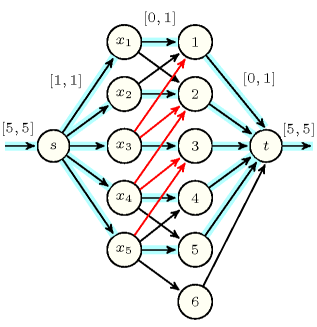
\includegraphics[width=45mm]{images/flow_alldiff_only_graph.png} \\
    \end{column}
    \begin{column}{0.7\textwidth}
      Using a flow model for \cons{AllDifferent}{} propagation
      \begin{itemize}
        \item feasible flows in the flow model = solutions to the constraint \vfill
        \item detect arcs that cannot carry flow in any feasible solutions $\rightarrow$ remove values from the domains of variables \vfill
        \item \textcolor{figblue}{Blue} arcs represent a maximal matching, \textcolor{red}{red} arcs represent infeasible arcs \vfill
        \item \textbf{Detect inconsistency early}: flow from (some) variables \textcolor{red}{cannot} be directed through the available values
        \begin{itemize}
          \item Not detected early through binary constraints \vfill
        \end{itemize}
      \end{itemize}
    \end{column}
  \end{columns}
\end{frame}

\begin{frame}{Linear decomposition of AllDifferent}
	\begin{columns}
		\begin{column}{0.2\textwidth}
		  \scalebox{0.7}{%	
			\begin{tikzpicture}[
				scale=0.6,
				every node/.style={circle, draw, minimum size=6mm, font=\small, inner sep=0pt},
				every edge/.style={draw, thick, -{Stealth[length=2mm,width=1.3mm]}},
				node distance=0.15cm and 1cm
				]
				
				% Nodes
				\node (X1) at (0,2.5) {$X_1$};
				\node (X2) at (0,1.25) {$X_2$};
				\node (X3) at (0,0) {$X_3$};
				\node (X4) at (0,-1.25) {$X_4$};
				\node (X5) at (0,-2.5) {$X_5$};
				
				\node[right=2.5cm of X1, yshift=0.5cm] (1) {1};
				\node[below=of 1] (2) {2};
				\node[below=of 2] (3) {3};
				\node[below=of 3] (4) {4};
				\node[below=of 4] (5) {5};
				\node[below=of 5] (6) {6};
				
				% Edges between X and numbered nodes
				\draw[black, thick, ->] (X1) -- (1);
				\draw[black, thick, ->] (X1) -- (2);
				
				\draw[black, thick, ->] (X2) -- (1);
				\draw[black, thick, ->] (X2) -- (2);
				
				\draw[black, thick, ->] (X3) -- (1);
				\draw[black, thick, ->] (X3) -- (2);
				\draw[black, thick, ->] (X3) -- (3);
				
				\draw[black, thick, ->] (X4) -- (2);
				\draw[black, thick, ->] (X4) -- (3);
				\draw[black, thick, ->] (X4) -- (4);
				\draw[black, thick, ->] (X4) -- (5);
				
				\draw[black, thick, ->] (X5) -- (3);
				\draw[black, thick, ->] (X5) -- (4);
				\draw[black, thick, ->] (X5) -- (5);
				\draw[black, thick, ->] (X5) -- (6);
				
			\end{tikzpicture}
		 }	
		\end{column}
		\begin{column}{0.8\textwidth}
			There is a natural \textit{linear} decomposition that corresponds to the bipartite matching formulation (and the flow graph):
			\vfill

			Each arc $(X_i,v)$ corresponds to the expression $(X_i = v)$:
			true when decision variable $X_i$ takes value $v$, false otherwise.
			Let $V = \bigcup_{X_i \in X} D(X_i)$.\vspace{-0.75em}
			\[
				\sum_{X_i \in X} \Iverson{X_i = v} \leq 1
					\quad \forall v \in V
					\qquad\text{(each value used at most once)\footnotemark}
			\]
			\footnotetext{An integer variable already takes exactly one domain value,
			so $\sum_{v \in D(X_i)}\Iverson{X_i = v} = 1$ needs no constraint.}
			\vfill
			
			While this is an efficient, more linear-friendly decomposition than the integer $\neq$ decomposition, it leads to weaker propagation than the global propagator that actively searches for unreachable arcs.
		\end{column}
	\end{columns}
\end{frame}

\begin{flashcardcpmpy}
\begin{frame}[fragile]{Linear decomposition of AllDifferent -- CPMpy}
  Let $V = \bigcup_{X_i \in X} D(X_i)$.
  \begin{center}
    \begin{tabular}{@{}ll@{}}
      \textbf{Math:} &
      $\displaystyle
        \sum_{X_i \in X} \Iverson{X_i = v} \leq 1
        \quad\forall v \in V
      $
      \\
      &
      {\small
        Iverson brackets $\Iverson{\cdot}$ turn a true/false condition into a number:
        $1$ if it holds, $0$ if not.
      }
      \\
      \textbf{CPMpy:} &
      \begin{minipage}[t]{0.75\linewidth}
        \vspace{-0.5em}
        \begin{lstlisting}[language=cpmpy,basicstyle=\small]
for v in V:
    m.add( cp.sum(xi == v for xi in X) <= 1 )\end{lstlisting}
      \end{minipage}
    \end{tabular}
  \end{center}
  \vfill
  Note how in math we write $X_i = v$ (single equality sign) and need Iverson brackets when writing Boolean expressions in mathematical operators; \\
  In CPMpy we write \cpminline{xi == v} (double equality sign) and \cpminline{cp.sum(...)} is also defined on Boolean expressions.
\end{frame}
\end{flashcardcpmpy}

\begin{frame}{\cons{NValueEq}{}}
	\begin{definition}[Pachet and Roy, 1999]
		The \cons{NValueEq}{X, res} functional global constraint holds if and only if \\ 
		the number of \textit{unique} values taken inside array $X$ is equal to $res$. 
		
		$ $
		
		If the argument $X$ is a 1-dimensional array of length $n$, then this means:\vspace{-0.75em}
		\[ \Cardinality{\Set{X_1,\dots,X_{n}}} = res \]
	\end{definition}
	\vfill
	
	Let $V$ be the set of unique values in the domains of $X$. \\
	The \defined{decomposition} creates an auxiliary Boolean variable $B_v$, indicating if that value is used, and constrains their count:
	\begin{align*}
		&B_v = \bigvee_{i} ( X_i = v ) &\forall v \in V \\
		&res = \sum_{v} B_v &
	\end{align*}
\end{frame}

\begin{frame}{\cons{NValueEq}{} example}
	\begin{center}
		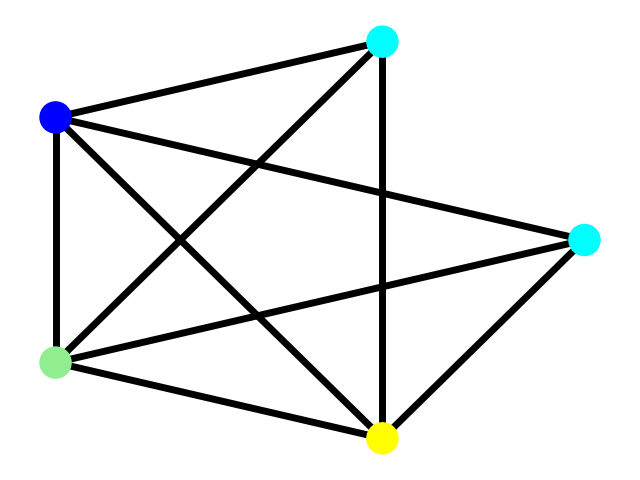
\includegraphics[height=25mm]{images/graph1.png}
	\end{center}
	
	\begin{example}
		Graph colouring: Neighbouring nodes must be given distinct colours + minimize the number of colours, i.e., minimize the number of \emph{unique} values used:
		\begin{align*}        
			&\text{node}_{1} \neq \text{node}_{2}, &\forall (\text{node}_1, \text{node}_2) \in \text{Edges} \\
			&\cons{NValueEq}{\text{nodes}, res} &\\
			&\minimize res &
		\end{align*}
	\end{example}
\end{frame}

\begin{flashcardcpmpy}
\begin{frame}{\cons{NValueEq}{} example -- CPMpy}
	\begin{center}
		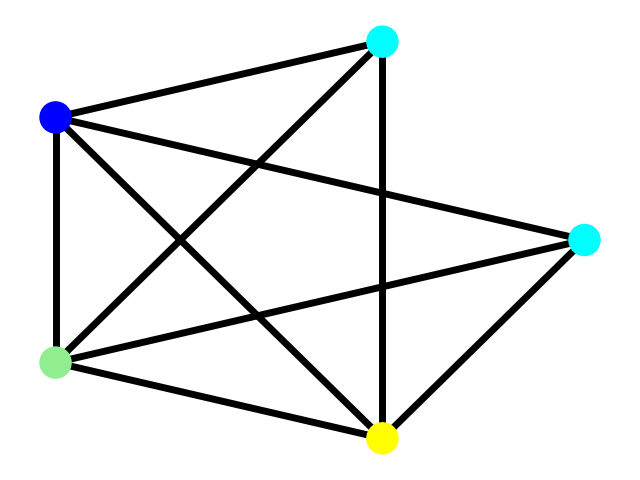
\includegraphics[height=25mm]{images/graph1.png}
	\end{center}
	
	\begin{example}
		Graph colouring: Neighbouring nodes must be given distinct colours + minimize the number of colours, i.e., minimize the number of \emph{unique} values used:
		\lstinputlisting[language=cpmpy,basicstyle=\small,firstline=12,lastline=15]{models_cpmpy/t4_nvalue.py}
	\end{example}
\end{frame}
\end{flashcardcpmpy}

\begin{frame}{\cons{NValueEq}{} vs \cons{AllDifferent}{}}
	Recap \cons{NValueEq}{}: if the argument $X$ is a 1-dimensional array of length $n$, then \cons{NValueEq}{X, res} expresses:\vspace{-0.75em}
	\[ \Cardinality{\Set{X_1,\dots,X_{n}}} = res \]
	\vfill
	
	If $res = n$ (the \emph{length} of array $X$), then \cons{NValueEq}{X, res} is equivalent to \cons{AllDifferent}{X}.
	\vfill
	
	Note, the decomposition would needlessly create the auxiliary $B_v$ variables (while we don't need $\bigvee_{i} ( X_i = v )$ as we know a value will either not be used, or be used exactly once).
	\vfill
	
	\textbf{In general,} always use the most specific available constraint predicate!
\end{frame}

\subsection{\cons{CountEq}{} and \cons{GlobalCardinalityCount}{}}


\begin{frame}{\cons{CountEq}{}}
	\begin{definition}
		The \cons{CountEq}{X, val, res} functional global constraint holds if and only if the number of \textit{occurrences} of value $val$ in array $X$ is equal to $res$.
	\end{definition}
	\vfill
	
	Note: $val$ can also be a decision variable (the constraint will hold for its value).
	\vfill
	
	The \defined{decomposition} is the following:
	\begin{align*}
		&res = \sum_{i} \Iverson{X_i = val} &
	\end{align*}
	
	\begin{examples}
	  $\cons{Count}{[1,1,2,3,2], 1} = 2, ~ \cons{Count}{[1,1,2,3,2], 3} = 1$
	  \begin{itemize}
	    \item Doctor rostering, Job allocation, Timetabling, \dots
	  \end{itemize}
	\end{examples}
\end{frame}


\begin{flashcardcpmpy}
\begin{frame}{\cons{CountEq}{} -- CPMpy}
	\begin{definition}
		The \cons{CountEq}{X, val, res} functional global constraint holds if and only if the number of \textit{occurrences} of value $val$ in array $X$ is equal to $res$.
	\end{definition}
	\vfill
	
	Note: $val$ can also be a decision variable (the constraint will hold for its value).
	\vfill
	
	The \defined{decomposition} is the following:
	\begin{center}
	  \cpminline{res == cp.sum(X == val)}
	\end{center}
	\vfill
	
	\begin{examples}
		\begin{itemize}
			\item Doctor rostering, Job allocation, Timetabling, \dots
		\end{itemize}
	\end{examples}
\end{frame}
\end{flashcardcpmpy}

\begin{flashcardcpmpy}
	\begin{frame}{\cons{CountEq}{} example -- CPMpy}
		\begin{example}[CPMpy model for our doctor rostering (indexing offset 0)]
			\vspace{-3mm}
			\lstinputlisting[language=cpmpy,firstline=9,lastline=26]{models_cpmpy/T01_doctor.py}
			\vspace{-3mm}
		\end{example}  
	\end{frame}
\end{flashcardcpmpy}

\begin{frame}{\cons{GlobalCardinalityCount}{}}
  What if you want to count multiple values at once?
	
  \begin{definition}[R\'{e}gin, 1996]
  	The \cons{GlobalCardinalityCount}{X, Vals, Res} global constraint holds if and only if for each value $Vals_i$, the number of occurrences in array $X$ is equal to $Res_i$.
  \end{definition}
  \vfill
  
  Note: $Vals$ can also be an array of decision variables.
  \vfill
  
  The \defined{decomposition} is the following:
  \begin{align*}
  	&\cons{CountEq}{X, Vals_i, Res_i} & \forall i \in \{1, \ldots, |Vals|\}
  \end{align*}
  \vfill
  
  Q: Why/when is it better to use GCC over Count?
  \pause
  
  \begin{examples}
  \begin{itemize}
  	\item Nurse rostering, facility location, car sequencing, \dots
  \end{itemize}
  \end{examples}
\end{frame}

\iffalse % Not used in 2025-2026
\begin{frame}{Facility Location}
  \vspace{-1.5em}
  \begin{columns}
    \begin{column}{0.6\textwidth}
      Warehouse location: we want to find which customers each warehouse will serve
    \end{column}
    \begin{column}{0.4\textwidth}
      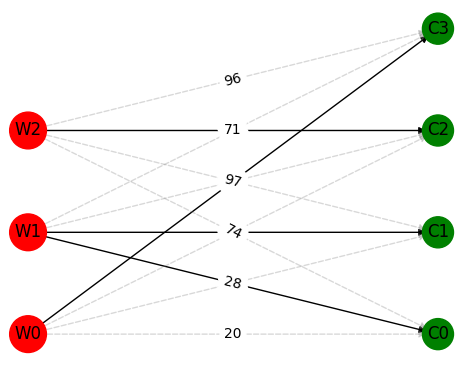
\includegraphics[width=40mm]{images/warehouse_plot.png} \\
    \end{column}
  \end{columns}

  \begin{example}
    \vfill
    Use the \cons{GlobalCardinalityCount}{assignments, warehouses, capacities} constraint to ensure that each warehouse is assigned the correct number of customers.
    \vfill
  \end{example}

  \alert{\cons{GlobalCardinalityCount}{} defines the exact number of occurrences, not a bound, i.e. takes capacity for each variable} \\ \vfill

  \blue{But every argument can be a variable! So, you can use variables (with the specified bounds) as capacities}
\end{frame}

\begin{flashcardcpmpy}
\begin{frame}{Facility Location -- CPMpy}
  \vspace{-1.5em}
  \begin{columns}
    \begin{column}{0.6\textwidth}
      Warehouse location: we want to find which customers each warehouse will serve
    \end{column}
    \begin{column}{0.4\textwidth}
      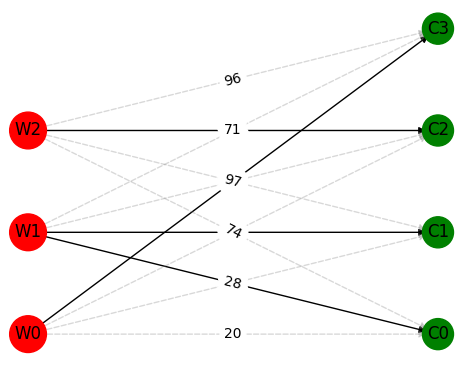
\includegraphics[width=40mm]{images/warehouse_plot.png} \\
    \end{column}
  \end{columns}

  \begin{example}[CPMpy]
    \vspace{-0.5em}
    \footnotesize
    \lstinputlisting[language=cpmpy,basicstyle=\small,firstline=13,lastline=14]{models_cpmpy/t4_gcc.py}
    \vspace{-0.5em}
  \end{example}

  \alert{\cons{GlobalCardinalityCount}{} defines the exact nr of occurrences, not a bound} \\ \vfill
  \blue{But every argument can be a variable! So, you can use variables (with the specified bounds) as capacities}
\end{frame}
\end{flashcardcpmpy}
\fi


\section{Scheduling}

\begin{frame}
	\begin{example}[Scheduling aircraft assembly transports (Airbus)]
		\begin{center}
			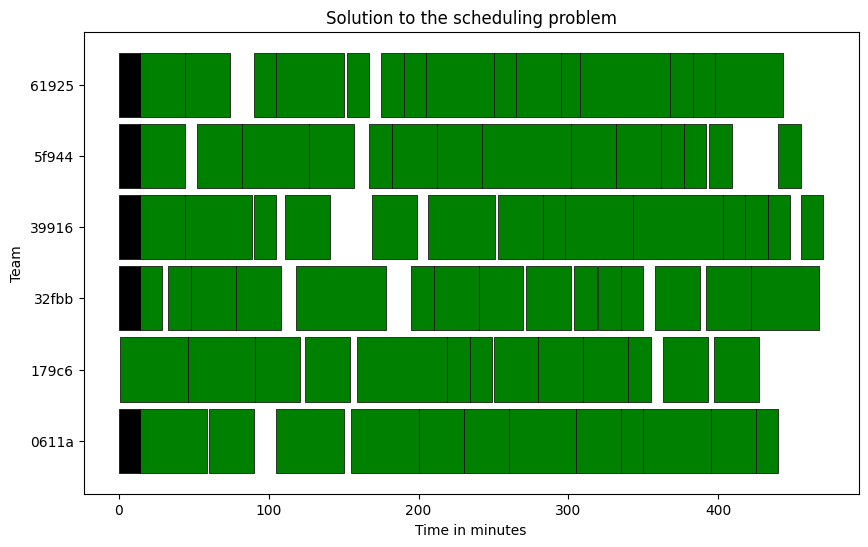
\includegraphics[height=35mm]{images/gantt}    
		\end{center}
		
		\textbf{Constraints} to be \textbf{satisfied}:
		\begin{enumerate}
			\item Each task has a pre-determined duration and allowed time-window
			\item Each task can only be handled by a subset of worker teams
			\item Some tasks have \textit{precedence} relations (e.g. same aircraft)
			\item \dots
		\end{enumerate}
		
		\textbf{Objective function} to be \textbf{minimised}: \\
		Minimize number of teams needed, and the workload balance between teams.
	\end{example}
\end{frame}

\begin{frame}{Scheduling tasks}
	Scheduling involves \textit{allocating tasks in time}. %, subject to constraints and an objective.
	\vfill
	
	In time = tasks should have a start-time and an end-time (and hence a duration).
	\vfill
	
	\begin{definition}[Task]
		A task $T$ is defined as a tuple $T = \langle s, d \rangle$ where:
		\begin{itemize}
			\item $s$ is the starting time of task $T$
			\item $d$ is the duration of task $T$
		\end{itemize}
		One can compute the time when it has just ended as $e = s + d$. %If its duration is a given constant, the task is fully determined by its start time.
	\end{definition}
	\begin{center}
		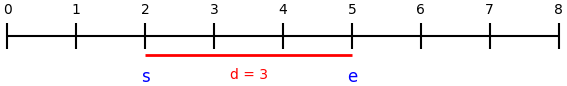
\includegraphics[height=30px]{images/task_time.png}
	\end{center}
	
	Some CP solvers have a special task decision variable, or even \textit{optional} task decision variables (e.g. if it can be executed by multiple teams/machines).
	\vfill
	
	%Tasks can have \textbf{constraints} on allowed start/end times, precedence requirements wrt other tasks, an amount of \textit{resource} that it consumes when executed, a subset of parallel machines on which it can run, ...
\end{frame}


\iffalse
% TODO: start with some simple predence graph?

\begin{frame}\label{ex:prec}
	\begin{definition}
		A \defined{precedence constraint} of task $T_1$ on task $T_2$
		requires \\ that~$T_1$ ends \alert{before} $T_2$ starts.  We say
		that task~$T_1$ \defined{precedes} task~$T_2$.
	\end{definition}
	\vfill
	
	\begin{example}[courtesy Magnus Rattfeldt]
		\begin{center}
			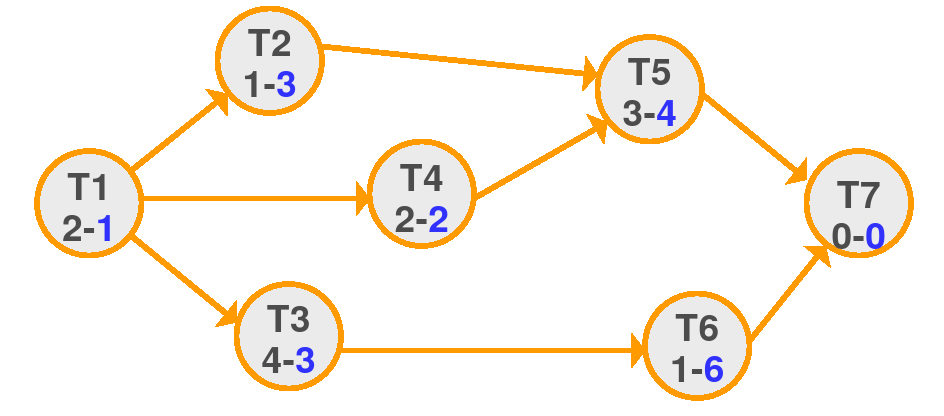
\includegraphics[width=80mm]{images/scheduling2} \\
			Sample tasks (circles), durations (black numbers), resource
			requirements (\blue{blue} numbers), and precedences
			(\textcolor{Orange}{orange} arrows).  Task~T7 is a dummy task,
			as we do not know which of tasks T5 and T6 will end last.
		\end{center}
	\end{example}
\end{frame}

\begin{frame}%{Scheduling precedences}
	Let us temporarily \textbf{ ignore the capacitated global reusable resource}: \\
	If we have an uncapacitated global reusable resource or each task
	has enough of its own local reusable resource, then the
	(polynomial-time-solvable problem) of \textbf{finding the earliest ending
		time, under only the precedence constraints}, for performing all the
	tasks can be modelled using linear inequalities.
	\vfill
	
	\begin{example}[continued]
		The precedence constraints indicated by the
		\textcolor{Orange}{orange} arrows on slide~\ref{ex:prec} are
		modelled as follows, based on the task durations indicated there
		in black: 
		
		\begin{align*}
			S_0 + D_0 \leq S_1, \quad S_0 + D_0 \leq S_2, \\ S_0 + D_0 \leq S_3, \quad S_1 + D_1 \leq S_4, \\ S_2 + D_2 \leq S_5, \quad S_3 + D_3 \leq S_4, \\ S_4 + D_4 \leq S_6, \quad S_5 + D_5 \leq S_6 \\
			\text{Minimize } S_6
		\end{align*} 
	\end{example}
\end{frame}

\begin{flashcardcpmpy}
	\begin{frame}%{Scheduling precedences -- CPMpy}
		Let us temporarily \textbf{ ignore the capacitated global reusable resource}: \\
		If we have an uncapacitated global reusable resource or each task
		has enough of its own local reusable resource, then the
		(polynomial-time-solvable problem) of \textbf{finding the earliest ending
			time, under only the precedence constraints}, for performing all the
		tasks can be modelled using linear inequalities.
		\vfill
		
		\begin{example}[continued]
			The precedence constraints indicated by the
			\textcolor{Orange}{orange} arrows on slide~\ref{ex:prec} are
			modelled as follows, based on the task durations indicated there
			in black: 
			
			\lstinputlisting[language=cpmpy,basicstyle=\small,firstline=8,lastline=13]{models_cpmpy/t4_precedence.py}
		\end{example}
	\end{frame}
\end{flashcardcpmpy}
\begin{flashcardminizinc}
	\begin{frame}[fragile]%{Scheduling precedences -- MiniZinc}
		Let us temporarily \textbf{ ignore the capacitated global reusable resource}: \\
		If we have an uncapacitated global reusable resource or each task
		has enough of its own local reusable resource, then the
		(polynomial-time-solvable problem) of \textbf{finding the earliest ending
			time, under only the precedence constraints}, for performing all the
		tasks can be modelled using linear inequalities.
		\vfill
		
		\begin{example}[continued]
			The precedence constraints indicated by the
			\textcolor{Orange}{orange} arrows on slide~\ref{ex:prec} are
			modelled as follows, based on the task durations indicated there
			in black: 
			
			\begin{mzn}
				constraint D = [2,1,4,2,3,1,0];
				constraint S[1]+D[1] <= S[2] /\ S[1]+D[1] <= S[3]
				/\ S[1]+D[1] <= S[4] /\ S[2]+D[2] <= S[5]
				/\ S[3]+D[3] <= S[6] /\ S[4]+D[4] <= S[5]
				/\ S[5]+D[5] <= S[7] /\ S[6]+D[6] <= S[7];
				% plug in here the resource constraint of the next slide
				solve minimize S[7];
			\end{mzn}
		\end{example}
	\end{frame}
\end{flashcardminizinc}
\fi

\subsection{\cons{NoOverlap}{}}

\begin{frame}{Scheduling with NoOverlap}
	Basic setting: schedule tasks for a \textit{single} team, where tasks can not overlap.
	\vfill
	
	\begin{definition}[Carlier, 1982]
		The \cons{NoOverlap}{S, D} global constraint, where each task $T_i$ has start-time $S_i$ and duration $D_i$, holds if and only if no two tasks $T_i$ and $T_j$ overlap in time.
		
		$ $
		
		Hence for every pair, either $T_i$ ends before $T_j$ starts, or $T_i$ starts after $T_j$ ends.
	\end{definition}
	\vfill
	
	The \defined{decomposition} is the following:
	\begin{align*}
		& ( S_i + D_i \leq S_j ) \vee ( S_j + D_j \leq S_i ) &\forall i, j \text{ with } i < j
	\end{align*}
	\vfill
	
	This constraint is also called the \texttt{Disjunctive} global constraint in the literature.
\end{frame}

\begin{flashcardcpmpy}
\begin{frame}{Scheduling with NoOverlap -- CPMpy}
	Basic setting: schedule tasks for a \textit{single} team, where tasks can not overlap.
	\vfill
	
	\begin{definition}[Carlier, 1982]
		The \cons{NoOverlap}{S, D} global constraint, where each task $T_i$ has start-time $S_i$ and duration $D_i$, holds if and only if no two tasks $T_i$ and $T_j$ overlap in time.
		
		$ $
		
		Hence for every pair, either $T_i$ ends before $T_j$ starts, or $T_i$ starts after $T_j$ ends.
	\end{definition}
	\vfill
	
	The \defined{decomposition} is pairwise non-overlap:
	\vfill
	%\begin{center}
		\cpminline{for i,j in all_pairs(range(n)):}\\
		\quad \cpminline{model += (S[i] + D[i] <= S[j]) | (S[j] + D[j] <= S[i])}
	%\end{center}
	\vfill
	
	This constraint is also called the \texttt{Disjunctive} global constraint in the literature.
\end{frame}
\end{flashcardcpmpy}


\subsection{\cons{Cumulative}{}}

\begin{frame}{Scheduling tasks}
	What if tasks \textit{can} overlap (e.g. be executed in parallel), but only up to some \textit{capacity limit} of the machine?
	\vfill
	
	\begin{center}
		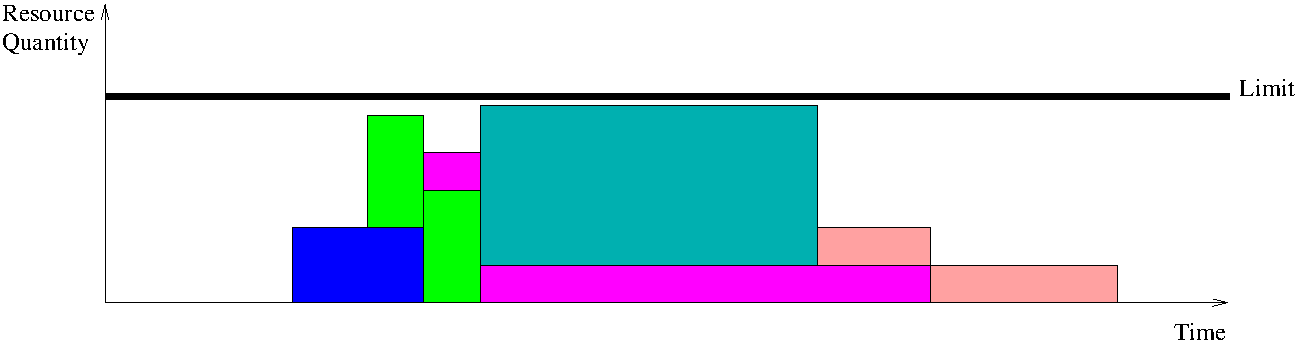
\includegraphics[width=100mm]{images/scheduling1} \\
		Fig: parallel tasks and a capacitated global reusable resource.
	\end{center}
	\vfill
	
	Requires the concept of \textit{resource usage} $R_i$ for each task $T_i$.
	
	\begin{examples}
		\begin{itemize}
			\item Memory use in cloud scheduling, room size in exam scheduling, oven capacity in metal processing, reservoir size in water management, \dots
		\end{itemize}
	\end{examples}
\end{frame}


\begin{frame}{\cons{Cumulative}{} resource use}
  \begin{definition}[Aggoun and Beldiceanu, 1993]
    The \cons{Cumulative}{S, D, R, c} global constraint, 
    where each task $T_i$ has start-time $S_i$,  duration $D_i$ and resource usage $R_i$, holds if and only if the total resource usage at any time does not exceed the capacity $c$.
  \end{definition}
  \vfill

  The time-based \defined{decomposition} is the following:
  \begin{align*}
  	& \sum_{i} R_i \cdot \Iverson{( S_i \leq t) \wedge ( t < S_i + D_i )} \leq c  & \forall t \in \{min(S_i) .. max(S_i+D_i)\}
  \end{align*}
  \vfill

  The task-based \defined{decomposition} is (only check each start time):
  \begin{align*}
  	& R_j + \sum_{i, i\neq j} R_i \cdot \Iverson{( S_i \leq S_j ) \wedge ( S_j < S_i + D_i )} \leq c   & \forall j
  \end{align*}
  \vfill

  \pause
  Q: If your solver does not have a \cons{Cumulative}{}, when should you use which decomposition?
\end{frame}
% TODO, make Boolean variables more explicit? (also in earlier slides)
%\begin{example}
%	\small
%	\cons{Cumulative}{s,d,r,c}:
%	Its time-resource decomposition introduces new Booleans \( B_{it} \), representing if task \( i \) (with start time $s_i$, and duration $d_i$) is active at time \( t \):
%	\vspace{-3mm}
%	\[
%	\forall t \in \{0..t_{\text{max}} - 1\}, \forall i \in \{1..n\} : \quad B_{it} \leftrightarrow (s_i \leq t) \land \neg(s_i \leq t - d_i)
%	\]
%	
%	The resource constraint at each time \( t \), for $n$ tasks, with $r_i$ being the resource consumption of task $i$, is expressed as:
%	\vspace{-3mm}
%	\[
%	\forall t \in \{0..t_{\text{max}} - 1\} : \quad \sum_{i \in [1..n]} r_i \cdot B_{it} \leq c
%	\]
%	\vspace{-3mm}
%\end{example}

\begin{frame}{Propagating \cons{Cumulative}{}, illustration\footnote{Images courtesy of Peter Stuckey}}
  \begin{columns}[t] % align at top
	% --- First pane ---
	\begin{column}{0.35\textwidth}
		For each task, determine \textit{compulsory time intervals}:
		
		$ $
		
		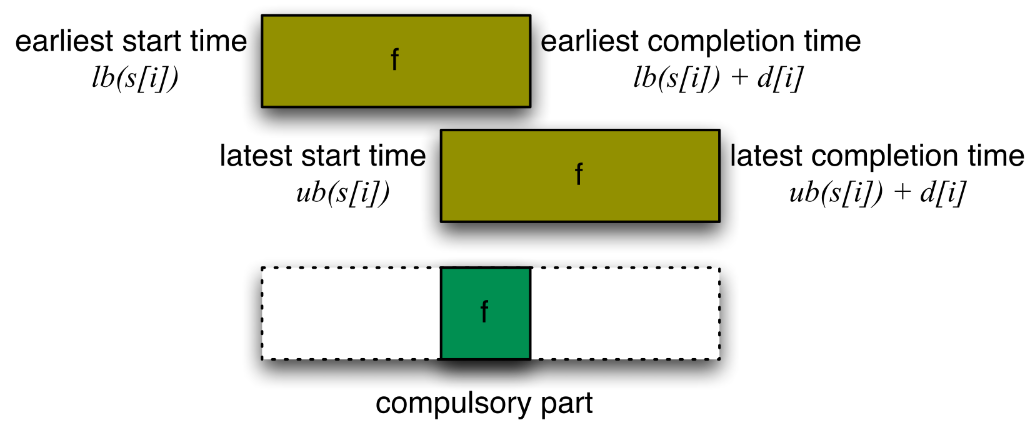
\includegraphics[width=\textwidth]{images/cumulative_compulsory.png}
	\end{column}
	
	% --- Second pane ---
	\begin{column}{0.3\textwidth}
		Fail if too much compulsory usage at some time interval:
		
		$ $
		
		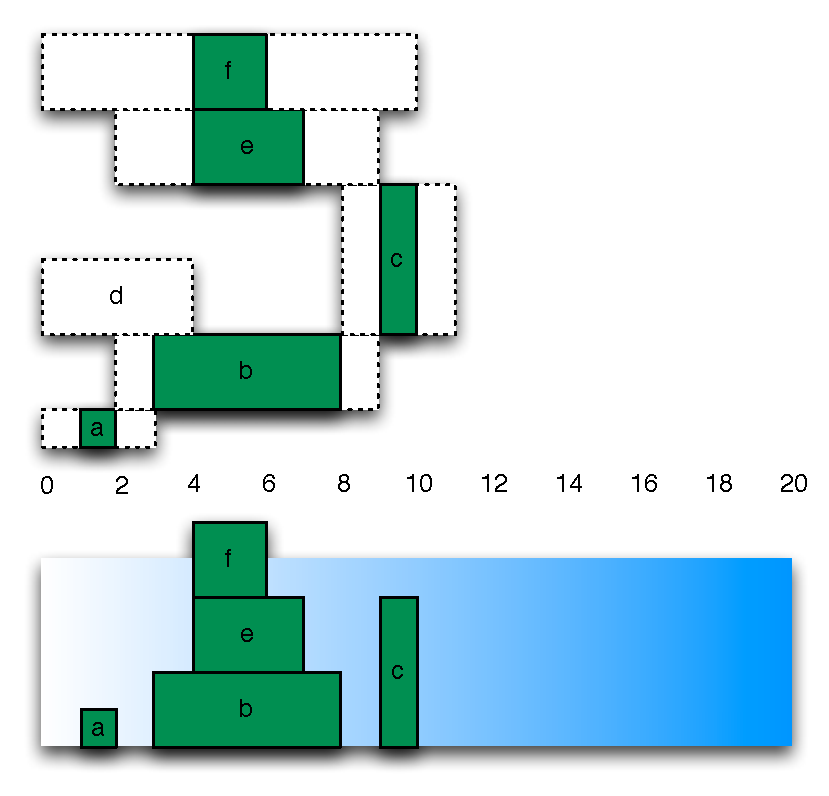
\includegraphics[width=\textwidth]{images/cumulative_consistency.pdf}
	\end{column}
	
	% --- Third pane ---
	\begin{column}{0.3\textwidth}
		Reduce start/end times based on compulsory intervals and capacity:
		
		$ $
		
		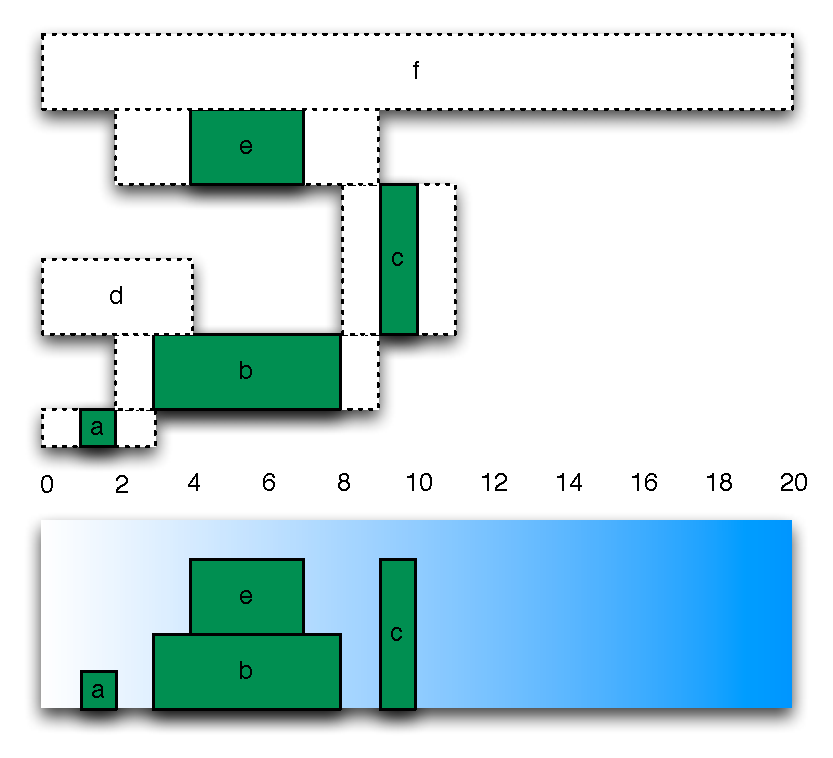
\includegraphics[width=\textwidth]{images/cumulative_timetable.pdf}
	\end{column}
  \end{columns}
\end{frame}

\begin{frame}{Propagating \cons{Cumulative}{}}
	The goal of the propagator is to ensure that
	\[
	\sum_i R_i \cdot \Iverson{S_i \leq t < S_i + D_i} \leq c
	\]
	holds for all times~$t$, \emph{without explicitly enumerating each~$t$}.
	\vfill
	
	\begin{itemize}
		\item \textbf{Core idea:} reason about \emph{time intervals} and \emph{task overlaps}
		\begin{itemize}
			\item Compute \defined{compulsory usage}: intervals of a task where it must occur in any feasible schedule
			\item Use these to determine intervals where capacity is partially consumed
		\end{itemize}
		\vfill
		
		\item \textbf{Propagation steps:}
		\begin{enumerate}
			\item Detect overload: if the sum of compulsory usages in an interval exceeds~$c$, fail.
			\item Tighten start and end times using reasoning on compulsory intervals, duration and remaining capacity.
			\item Optionally use \defined{edge-finding} or \defined{energetic reasoning} for stronger pruning.
		\end{enumerate}
	\end{itemize}
\end{frame}


% TODO: relation NoOverlap - Cumulative
%Can be also modeled as: \cons{Cumulative}{S, D, [1, 1, \ldots, 1], 1}
%\alert{Always use the most specific available constraint predicate!}
\begin{frame}{Global constraint relations}
	
	\[
	\cons{Cumulative}{S, D, [1, 1, \ldots, 1], 1} = 
	\only<1>{?}
	\only<2->{\cons{NoOverlap}{S, D}}
	\]
	\vfill
		
	\only<2->{
	\[
	\cons{Cumulative}{S, [1, 1, \ldots, 1], [1, 1, \ldots, 1], 1} = 
	\only<2>{?}
	\only<3->{\cons{NoOverlap}{S, [1, 1, \ldots, 1]}
	\]
	\[
	 = \cons{AllDifferent}{S}}
	\]
	\vfill	
	}
	
	\only<3->{\textbf{In general,} always use the most specific available constraint predicate!}
\end{frame}

\section{Routing}
\subsection{\cons{Circuit}{}}

\begin{frame}{Enabling the representation of a circuit in a digraph}
	\begin{itemize}
		\item Let decision variable $S_v$ denote the successor of vertex $v$ in the circuit.
		\item The domain of $S_v$ is the set of vertices to which there is an arc from vertex $v$.
	\end{itemize}
	\begin{definition}[Laurière, 1978; Beldiceanu and Contejean, 1994]
		The \cons{Circuit}{S} global constraint holds if and only if $\forall ~ v$ the arcs $v \rightarrow S_v$ form a Hamiltonian circuit: each vertex is visited exactly once.
	\end{definition}
	
	\begin{example}[Vehicle Routing]
		\begin{columns}
			\begin{column}{0.4\textwidth}
				\centering
				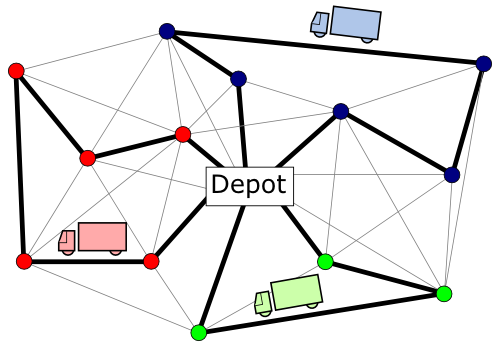
\includegraphics[width=40mm]{images/VRP.png}
			\end{column}
			\begin{column}{0.6\textwidth}
				\begin{itemize}
					\item Find optimal routes for multiple vehicles visiting a set of locations.
					\item 1 vehicle = Traveling Salesman Problem.
				\end{itemize}
			\end{column}
		\end{columns}
	\end{example}
\end{frame}

\begin{frame}
	\begin{example}[Vehicle routing]
		
		\begin{columns}
			\begin{column}{0.4\textwidth}        
				\centering
				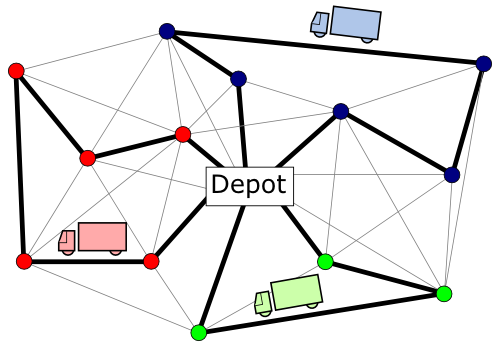
\includegraphics[width=40mm]{images/VRP.png} \\
			\end{column}
			\begin{column}{0.6\textwidth}        
				\begin{itemize}
					\item Find optimal routes for multiple vehicles visiting a set of locations
					\item 1 vehicle = Traveling Salesman Problem
				\end{itemize}
			\end{column}
		\end{columns}
	\end{example}
	
	Travelling salesman problem (generalise this for vehicle
	routing problems with multiple vehicles or with side constraints):
	
	\[
	\text{Circuit}(S)
	\]
	\[
	\text{Minimize} \quad \sum_{v=0}^{n-1} \text{distance}(v, S_v)
	\]   
\end{frame}

\begin{flashcardcpmpy}
	\begin{frame}
		\begin{example}[Vehicle routing]
			
			\begin{columns}
				\begin{column}{0.4\textwidth}        
					\centering
					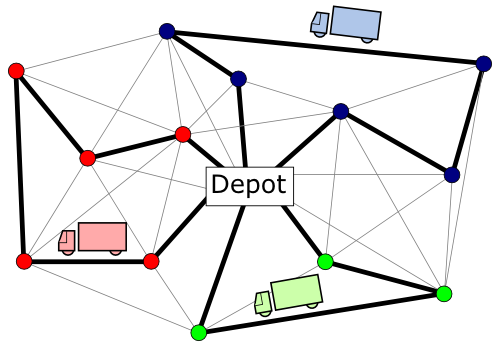
\includegraphics[width=40mm]{images/VRP.png} \\
				\end{column}
				\begin{column}{0.6\textwidth}        
					\begin{itemize}
						\item Find optimal routes for multiple vehicles visiting a set of locations
						\item 1 vehicle = Traveling Salesman Problem
					\end{itemize}
				\end{column}
			\end{columns}
		\end{example}
		
		Travelling salesman problem (generalise this for vehicle
		routing problems with multiple vehicles or with side constraints):
		
		\begin{example}[CPMpy Circuit TSP (indexing offset 0)]
		\lstinputlisting[language=cpmpy,basicstyle=\small,firstline=11,lastline=15]{models_cpmpy/t4_circuit.py}
		\end{example}
		
	\end{frame}
\end{flashcardcpmpy}
\begin{flashcardminizinc}
	\begin{frame}
		\begin{example}[Vehicle routing]
			
			\begin{columns}
				\begin{column}{0.4\textwidth}        
					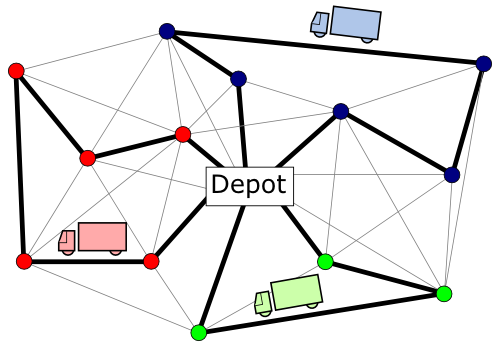
\includegraphics[width=60mm]{images/VRP.png} \\
				\end{column}
				\begin{column}{0.6\textwidth}        
					\begin{itemize}
						\item Find optimal routes for multiple vehicles visiting a set of locations
						\item 1 vehicle = Traveling Salesman Problem
					\end{itemize}
				\end{column}
			\end{columns}
			
			Travelling salesman problem (generalise this for vehicle
			routing problems with multiple vehicles or with side constraints):
			
			\vspace{-2mm}
			\lstinputlisting[language=Mzn,firstnumber=3,firstline=3,lastline=4]{models_minizinc/tsp.mzn}
			\vspace{-2mm}
			
			Requiring a \alert{directed path} from vertex \mzninline{v} to
			vertex \mzninline{w}: 
			\mzninline{constraint subcircuit(S) /\ S[w] = v;}
			upon adding \mzninline{v} to the domain of \mzninline{S[w]} if
			need be.
		\end{example}
		\vspace{-1mm}
		
		Many graph constraints, including \mzninline{dpath}, exist in
		\MiniZinc.
	\end{frame}
\end{flashcardminizinc}
% TODO: something more in-depth on this global constraint... the decomposition? maybe also even MTZ?

\section{Ad-hoc constraints over integer values}

\subsection{\cons{ElementEq}{}}

\begin{frame}{\cons{ElementEq}{}}
	Modeling an \textcolor{Melon}{unknown element of an array}: $Arr[x]$ where $x$ is a decision variable.
	\vfill
	
	\begin{example}[Job allocation at minimal salary cost]
		\structured{Given} the salaries of work applicants $Salary$ for different jobs, \\
		\structured{find} a work applicant
		for each job \structured{such that} some constraints (on the
		qualifications of the work applicants for the jobs, on workload
		distribution, etc) are satisfied and the \textbf{total salary cost is
			minimal}: 
		
		\begin{align*}
			&\text{workers}_j \in \{0, \dots, \text{Apps}-1\} &&\forall j \\
			&\text{total\_cost} = \sum_{j} \text{Salary}[\text{workers}_j]\\
			&\minimize \text{total\_cost}
		\end{align*}
		
		\vfill
		\alert{We do not know at modelling time the worker allocated to each job!}
	\end{example}
\end{frame}

\begin{flashcardcpmpy}
	\begin{frame}{\cons{ElementEq}{}}
		Modeling an \textcolor{Melon}{unknown element of an array}: $Arr[x]$ where $x$ is a decision variable.
		\vfill
		
		\begin{example}[Job allocation at minimal salary cost (indexing offset 0)]
			\structured{Given} the salaries of work applicants $Salary$ for different jobs, \\
			\structured{find} a work applicant
			for each job \structured{such that} some constraints (on the
			qualifications of the work applicants for the jobs, on workload
			distribution, etc) are satisfied and the \textbf{total salary cost is
				minimal}: 
			\vfill
			
			\lstinputlisting[language=cpmpy,basicstyle=\footnotesize,firstline=17,lastline=20,numbers=none]{models_cpmpy/t4_element.py} \vfill
			%Line~3 is equivalent to the less readable formulation: \\
			%\cpminline{total_cost = cp.sum([cp.Element(Salary, worker) for worker in workers])}
			\vfill
			
			\alert{We do not know at modelling time the worker allocated to each job!} \\ \vfill
			We need to express the relation between variables/expressions and values of arrays based on unknown indices \dots
		\end{example}
	\end{frame}
\end{flashcardcpmpy}

\begin{frame}{The \cons{ElementEq}{} Global Constraint}
	We need to express the relation between variables/expressions and values of arrays based on unknown indices \dots
	
	\begin{definition}[Van Hentenryck and Carillon, 1988]
		The \cons{ElementEq}{Arr, idx, res} functional global constraint holds if and only if $Arr[idx] = res$.
	\end{definition}\vfill
	
	\alert{For better model readability}, the \cons{ElementEq}{} predicate is typically not directly used,
	when modeling languages allow direct indexing; e.g. \texttt{res == Arr[idx]}
	even if \texttt{idx} is an integer expression involving at least one decision variable.
	\vfill
	
	Note that \cons{Element}{} can be multi-dimensional: \cpminline{Arr[idx1, idx2]}.
	%We assume that the indices can only take values \alert{within the bounds of the array.}
\end{frame}


\subsection{\con{Table}}

\begin{frame}{\con{Table}}
	\begin{definition}
		The \cons{Table}{X, T} constraint holds iff the values of array $X$ of decision variables form a row in the $n$-by-$|X|$ matrix $T$ of values.
		\parBreak
		
		Mathematically, $\exists \text{ row } \in T \text{ such that } \forall j, \, X_j = \text{row}_j$ %it restricts the values of the given variables in $X$ to combinations listed in the predefined table $T$.
	\end{definition}
	\only<1>{
	\begin{example}
		Assigning Workers $W_1, W_2$ to Shifts, but only the specific assignments are allowed:
		\[
		\text{T} = \{ (1, 2), (1, 3), (2, 3) \}
		\]
		
		The \cons{Table}{} constraint is applied as:
		\[
		\cons{Table}{[W_1, W_2], T}
		\]            
	\end{example}
	}
	\only<2>{
	%The 2D array $T$ provides an \defined{extensional definition} of the %constraint we impose. \\    
	One \defined{decomposition} creates a Boolean variable per row, enforcing at least one true:
	\begin{align*}
		&B_i \rightarrow \bigwedge_j ( X_j = T_{ij} ) & \forall i \\
		&\bigvee_i B_i & 
	\end{align*}

	An alternative \defined{decomposition} creates one integer decision variable $r \in \interval{1}{n}$ that represents the active row index, and posts an \con{Element} per $X$ variable/column:
	\begin{align*}
		&X_j = \cons{Element}{[T_{1j},\ldots,T_{nj}], r} & \forall j
	\end{align*}
	}
\end{frame}


%\subsection{\cons{Regular}{}}
%\begin{frame}{\cons{Regular}{}}
%TODO... regular + decomposition with repeating tables?
%\end{frame}

\section{Other global constraints}

\begin{frame}{Other global constraints}
	\begin{itemize}
		\item Non-linear arithmetic: \cons{MinimumEq}{}, \cons{MaximumEq}{}, \cons{AbsEq}{}
		\item Other Boolean operators: \cons{Xor}{}
		\item Other ad-hoc constraints: \cons{ShortTable}{}, \cons{NegativeTable}{}
		\item Symmetry breaking (later lecture): \cons{Increasing}{}, \cons{IncreasingStrict}{}, \cons{Decreasing}{}, \cons{DecreasingStrict}{}, \cons{LexLess}{}, \cons{LexLessEq}{}, \ldots
		\item and more
	\end{itemize}
	\vfill
	
	\textbf{CP modeling systems} allow you to define your own global constraints and corresponding decomposition (= like a helper function)
	\vfill
	
	\textbf{CP solvers} allow you to implement your own global constraints and corresponding propagator (= algorithms that speed up solving)
\end{frame}

\begin{frame}{Summary}
  Global Constraints: captures combinatorial substructure in the problem
    \vfill

  \begin{itemize}
  	\item Expressiveness: modeler can reuse existing building blocks \vfill
  	\item Efficiency: solvers with matching primitive constraints could perform better, because: 
  	\begin{itemize}
  		\item it might infer \textit{more} than the decomposition
  		\item it might avoid creating (many) auxiliary variables
  		\item it might use optimized data structures that make the check faster
  	\end{itemize} \vfill
  	\item Compatibility: for other solvers, a known (ideally well-performing) default decomposition will be used. Sometimes even different decompositions depending on the target solver. \\
  	Could be faster than what you would write!
  \end{itemize}
\end{frame}


\end{document}
